\chapter{Application and Case Studies}

As the previous chapters have shed light on the process of algorithmic and thermal design; mainly in theory, illustrating the basic concepts; this chapter will delve into the practical tools used in the process, which will facilitate input of algorithms into the modelling process. Afterwards, a showcase of previous experiments with algorithmic design by either performative or generative tools

\section{Algorithm and Value Entry}

\subsection{End-user Programming}

The term ``End-user'' is used to refer to the final user of the computer application. The programming input method for the end-user is called \emph{scripting}, which allows end-user to participate in the development of the programme to add unique functionality; therefore, transferring some of tasks traditionally assigned to the software developer to the end-user.

Although scripting allows end-users to introduce new functionality, it does not mean that users would be creating new software. Scripting allows end-users to access the underlying structure of existing software and embed new functionality in it. This type of input allows for extended expressive control and higher productivity in the design process. \cite{kashyap01}

Scripting is very similar to traditional programming procedure; entering a series of instructions written in computer code, and executed within the software environment. Some popular scripting languages and their corresponding model oriented software environments include: 

\begin{enumerate}
\item AutoLisp for AutoCAD
\item RhinoScript for Rhinoceros
\item MEL for Maya
\item MAXSCRIPT for 3DsMax
\end{enumerate}

\subsection{Parametric Modelling}

Parametric Modelling is a system where a 3D geometric model has parametric attributes subject to variation, modification is usually done through numerical input of the variable value (refer to section \ref{sec:GeoModel} on parametric modelling). The model is also built with constraints that ensure that some aspects of the model are not altered, or that some are automatically changed when others are in the process of parameter or variable value change. Parametric modelling offers flexibility of change to the design; the model in this case could be called a \emph{smart} CAD model \cite{kashyap01}.

Another form of parametric modelling is generative parametric graphical modules, which analyse and decompose geometry into elements which can be controlled as input and output data into processes which ultimately affect the model. A prominent example is Grasshopper plugin for Rhinoceros.

Parametric models are of great value to performative oriented design processes, which is sometimes fused with scripting, benefiting from both in speeding the process and achieving better results.

\clearpage
\section{Case Studies}

\subsection{Adaptable Responsive Architecture}

The following will showcase a number of experiments by Alejandro Zulas \cite{zulas04}, utilising scripting to create adaptable responsive enclosure systems with emphasis on sunlight incidence.

\subsubsection{The Mutable Curtain}

The author attempted the design of a box capable of modulating light going through it (fig. \ref{fig:AZulasEncl}), which was done using Rhinoceros modelling program and its scripting language; \emph{Rhinoscript}. The experiment was an attempt to create an adaptive, responsive enclosure system which responded to solar incidence angles. 

\begin{figure}[htbp]
\centering
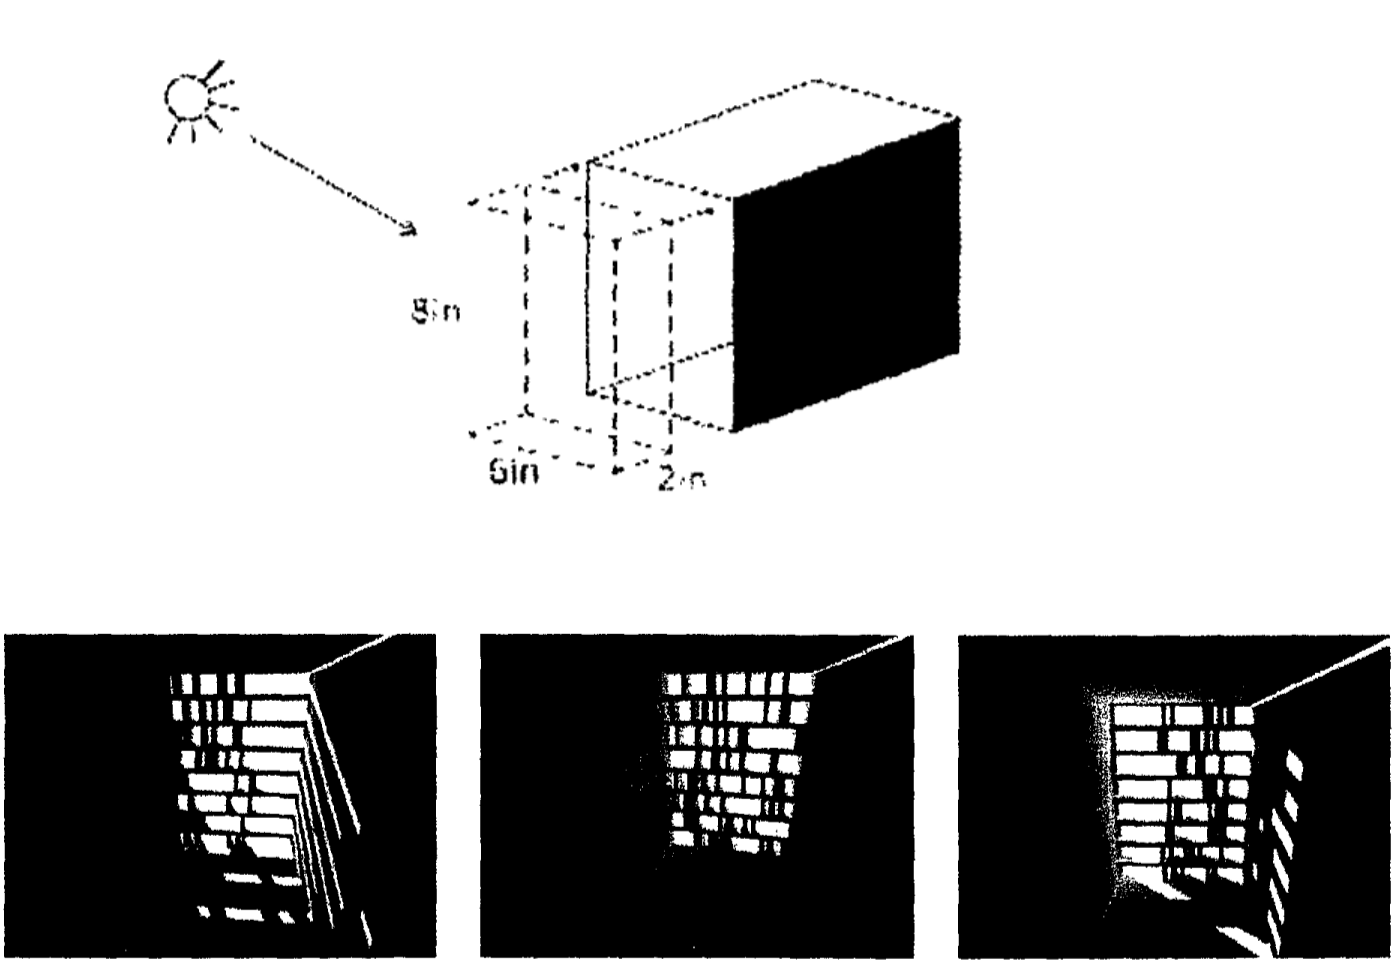
\includegraphics[width=\textwidth]{./Images/1-Enclosure}
\caption[Responsive Adaptable Enclosure Experiment]{The Enclosure and Results \cite{zulas04}}
\label{fig:AZulasEncl}
\end{figure}

The main variable in the experiment was the ratio of enclosure wall solid and void. Using an advanced draughting engine such Rhino and scripting language such as Rhinoscript, the researcher was able to create a responsive system with a generative random function to regulate the amount of light penetrating the enclosure (fig. \ref{fig:TransSeq}).


\begin{figure}[htbp]
\centering
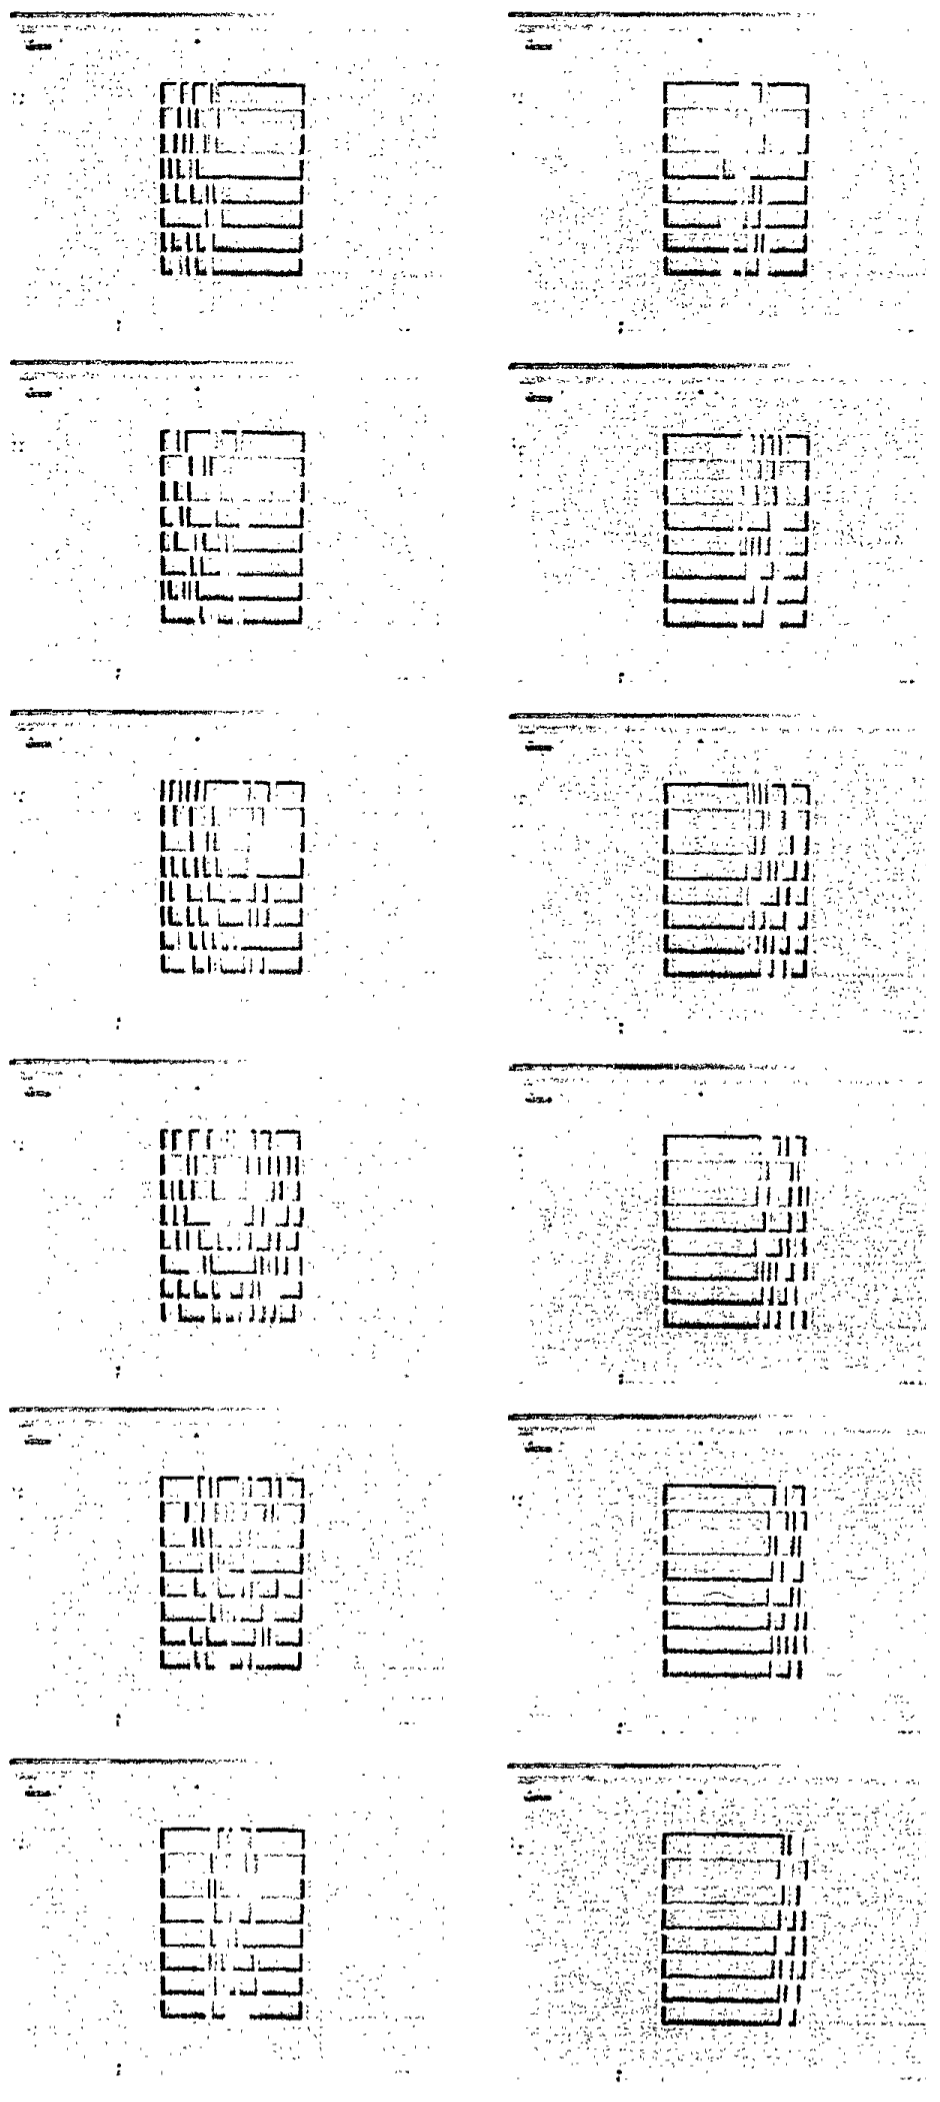
\includegraphics[height=17cm]{./Images/2-TransfSequ}
\caption[Transformation Sequence of Enclosure]{Transformation Sequence \cite{zulas04}}
\label{fig:TransSeq}
\end{figure}

\subsubsection{Responsive Louvres System}

Another experiment by the same author \cite{zulas04} was done using a parametric design driven program called CATIA (Computer Aided Three-Dimensional Interactive Application). The objective of this exercise was also to modulate light at the enclosure level, but through shading. The researcher used a number of vertical and horizontal louvres which responded to two factors; the location of the sun throughout days of different seasons which would affect the arrangement of the louvres, in addition to the angle of incidence which affected the orientation of each louvre as to reflect the light in a direction away from the building. 

The parametric CAD program, CATIA; had some advantages over Rhinoscript as it displayed the effect of any amendments to the script interactively in the form of graphical feedback, which was beneficial to the process. 

\subsubsection{Adaptable Pavilion}
\label{sec:AdptPav}

Another experiment using CATIA; an attempt to design a temporary exhibition pavilion \cite{zulas04}. The exercise focuses on the conception of a contextual responsive building addressing different variations on the overall building form and envelope in relation to sunlight. 

\begin{figure}[htbp]
\centering
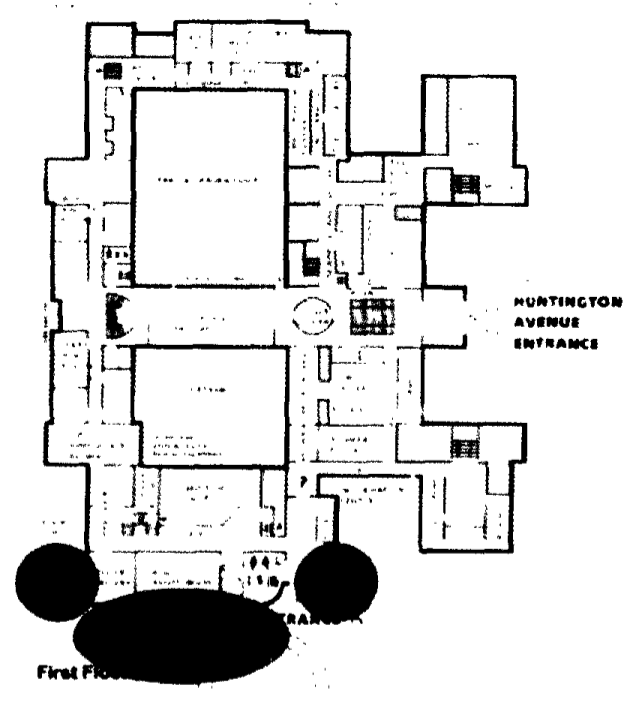
\includegraphics[width=0.5\textwidth]{./Images/4-Location}
\caption[Case Study Location]{Pavilion Location \cite{zulas04}}
\label{fig:PvlLoc}
\end{figure}

\paragraph{Design Intentions:} 

\begin{enumerate}
\item Generate an appropriate enclosed environment for the sculptures to be exhibited.
\item Implementation of a responsive louvre system as a filter to redirect light incidence inside the pavilion.
\item Analysing the behaviour of the building towards conceiving a sun responsive building (fig. \ref{fig:DesignInt}). 
\end{enumerate}

\begin{figure}[htbp]
\centering
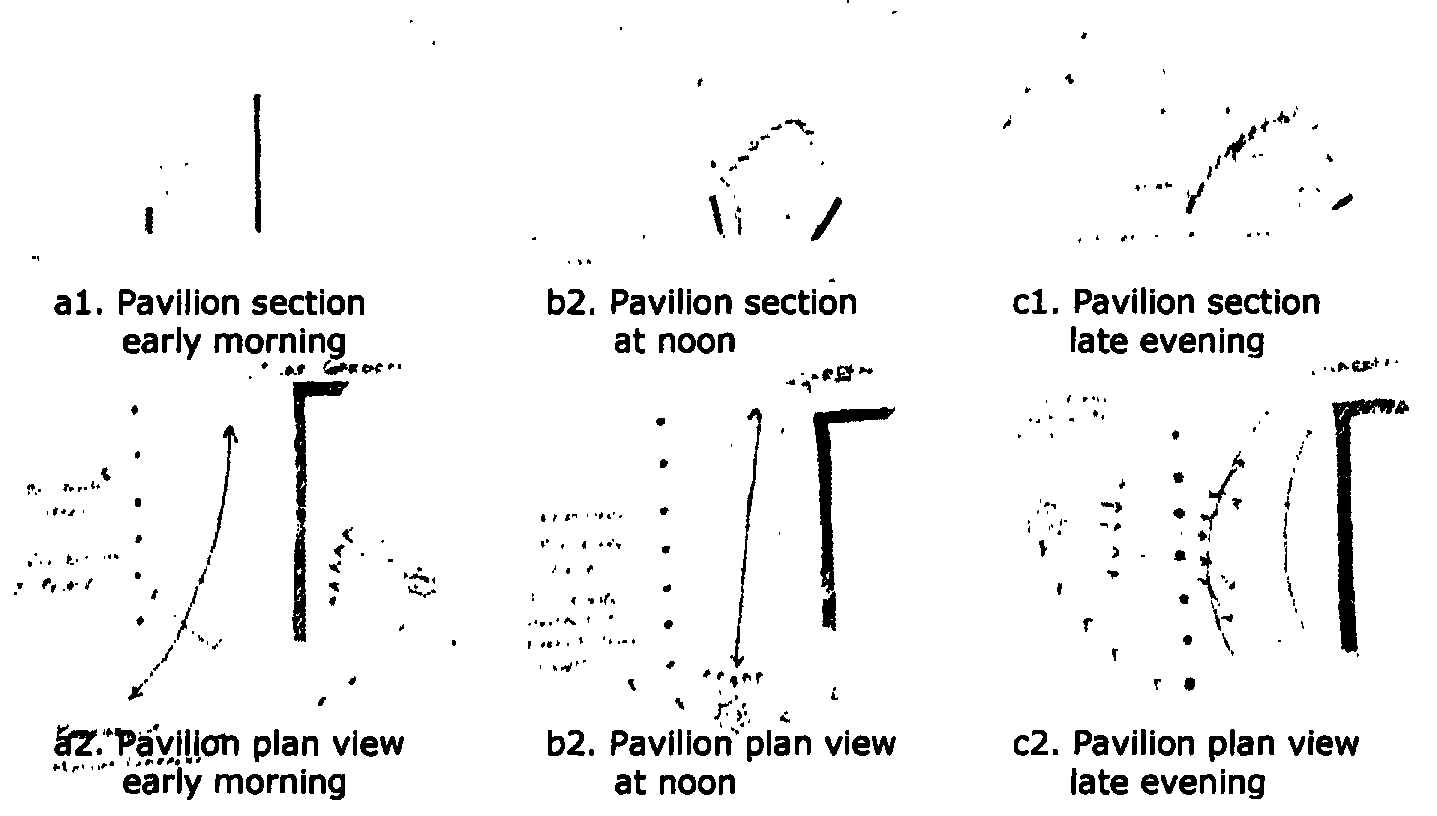
\includegraphics[width=\textwidth]{./Images/3-DesignIntent}
\caption[Pavilion Design Intentions]{Design Intentions \cite{zulas04}}
\label{fig:DesignInt}
\end{figure}

The context consisted of the sun, the museum wall and trees defining the yard. The museum wall and the trees were defined as static elements of the context, while the sun was understood as a dynamic element; this was to be taken into consideration as input. The main variables taken into consideration were the pavilions shape, length, height, proportions\ldots etc. 

Object relations were programmed using conditional ``\emph{if : then \dots else : that}''. In other words; \emph{if} the location of the sun in relation to its day-path is ``\emph{n}'', \emph{then} the line defining the pavilion's profile gets increased or decreased or rotated or thickened\ldots etc, by a predefined ``\emph{n}'' factor. (Refer to fig. \ref{fig:MpRlt})

\begin{figure}[htbp]
\centering
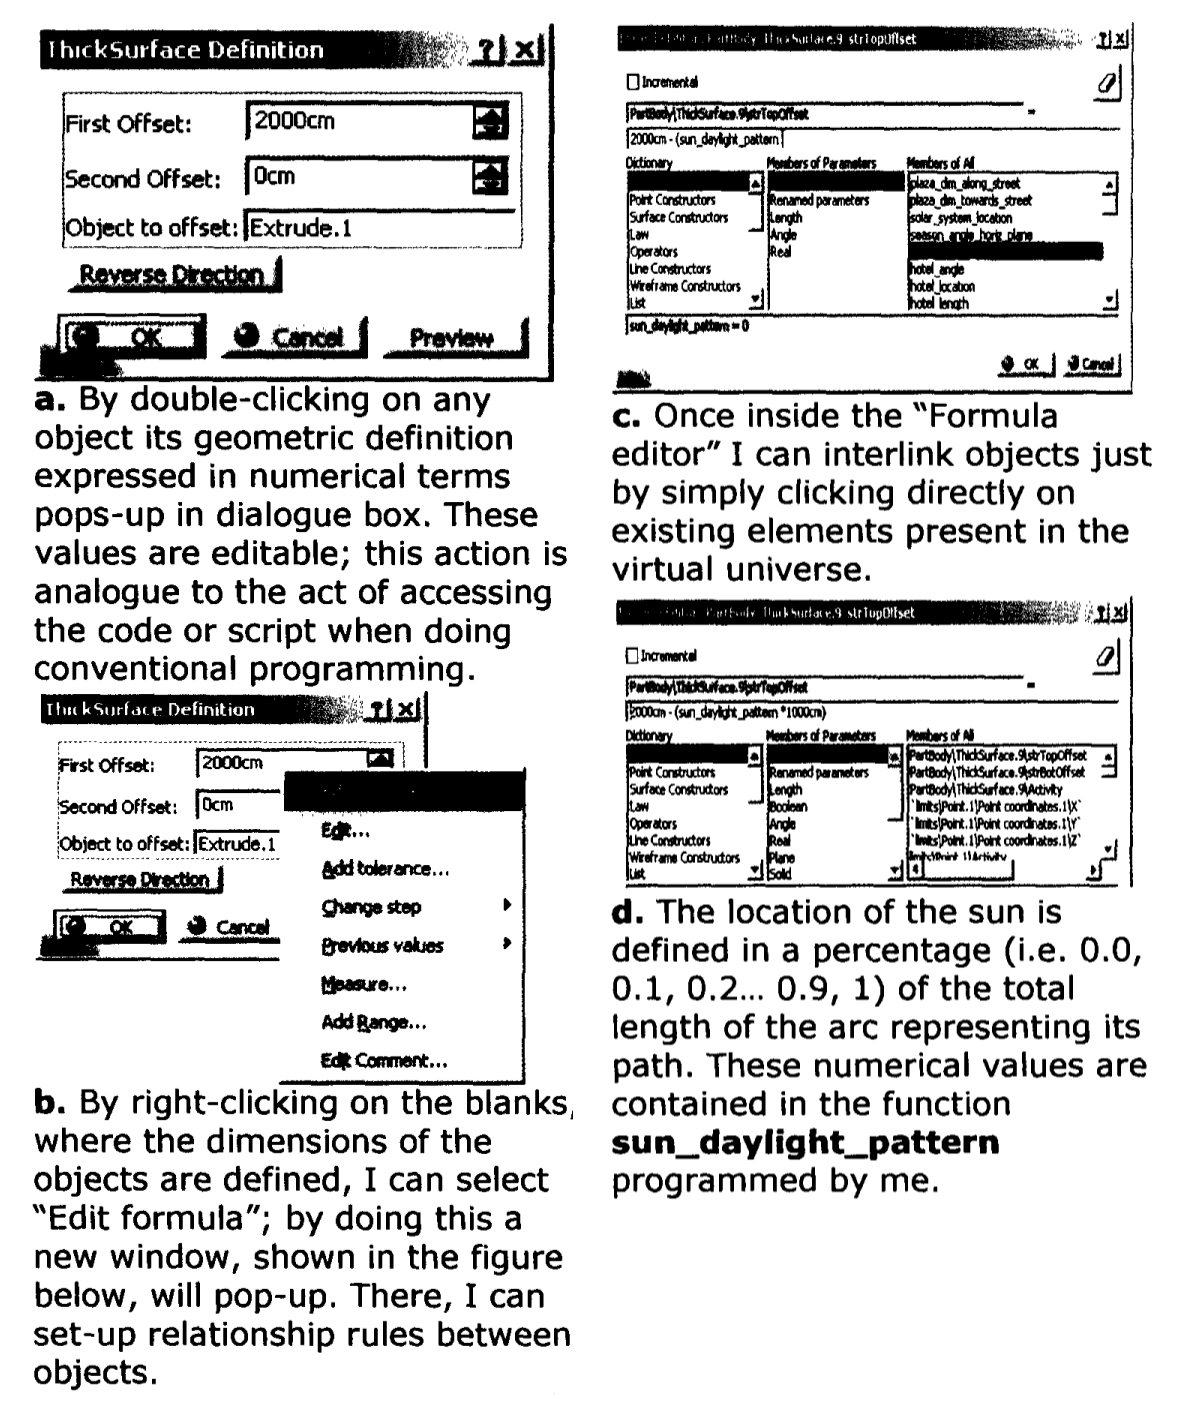
\includegraphics[width=\textwidth]{./Images/5-MappingRelations}
\caption[Mapping Design Relations]{Mapping Relationships \cite{zulas04}}
\label{fig:MpRlt}
\end{figure}

The interactiveness of CATIA was quite notable when the author attempted to change the location of the sun by means of a graphical slider and witnessed real-time changes to building shape due to the change in solar location (fig. \ref{fig:IntActCAT})

\begin{figure}[htbp]
\centering
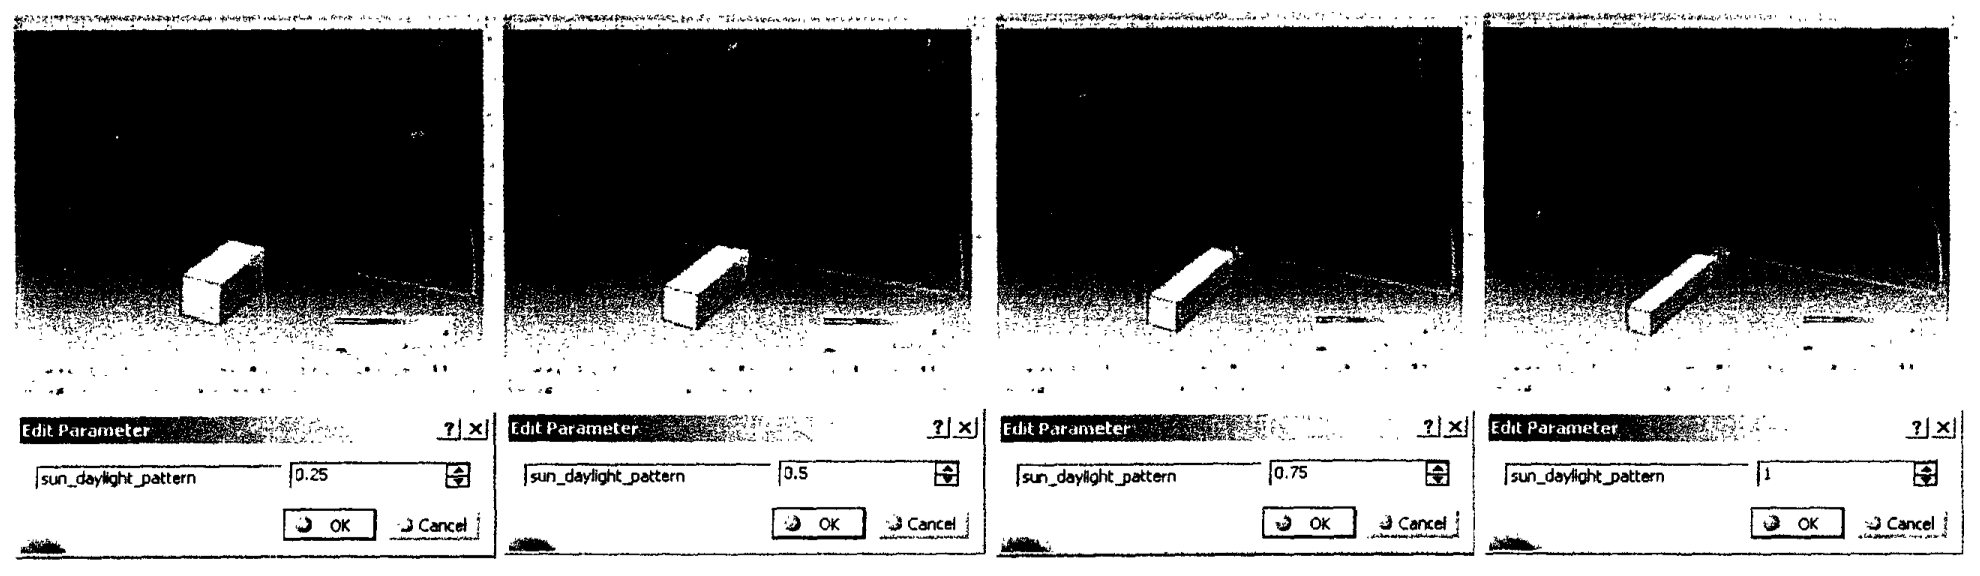
\includegraphics[width=\textwidth]{./Images/6-InteractiveCATIA}
\caption[Interactive Response]{Automated Adaption \cite{zulas04}}
\label{fig:IntActCAT}
\end{figure}

The end result was quite similar to the initial design intentions (fig. \ref{fig:FinalPav}).

\begin{figure}[htbp]
\centering
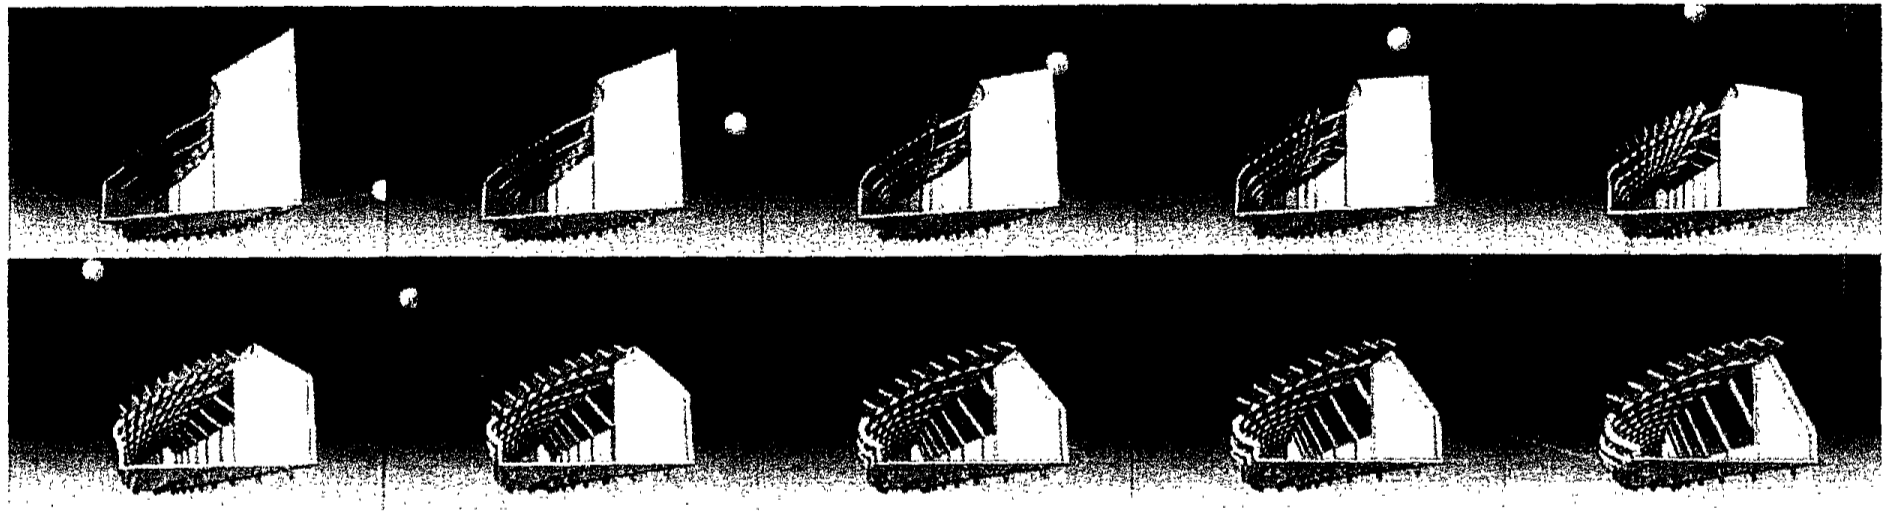
\includegraphics[width=\textwidth]{./Images/7-FinalPavilion}
\caption[Adaptable Pavilion Design Results]{The Adaptable Pavilion \cite{zulas04}}
\label{fig:FinalPav}
\end{figure}

\newpage
\subsubsection{The Kendall Pavilion}

The following is a comprehensive exercise to create an adaptable responsive system, with an approach combining the following concepts and control mechanisms:

\begin{enumerate}
\item Programming objects using Shape Grammar.
\item Conventional programming through coding or scripting.
\item Modelling a real-world situation corresponding to naturally occurring phenomena.
\end{enumerate}

The task is to design an architectural envelope capable of performing responsive geometrical reconfiguration based on the idea of adaption in relation to a geographical location, urban context, and to specific design intentions, responding to the designer's direct manipulation.

\paragraph{The Urban Context Description}

The space designated to locate the pavilion is surrounded by and high and medium sized structures.

\begin{figure}[htbp]
\centering
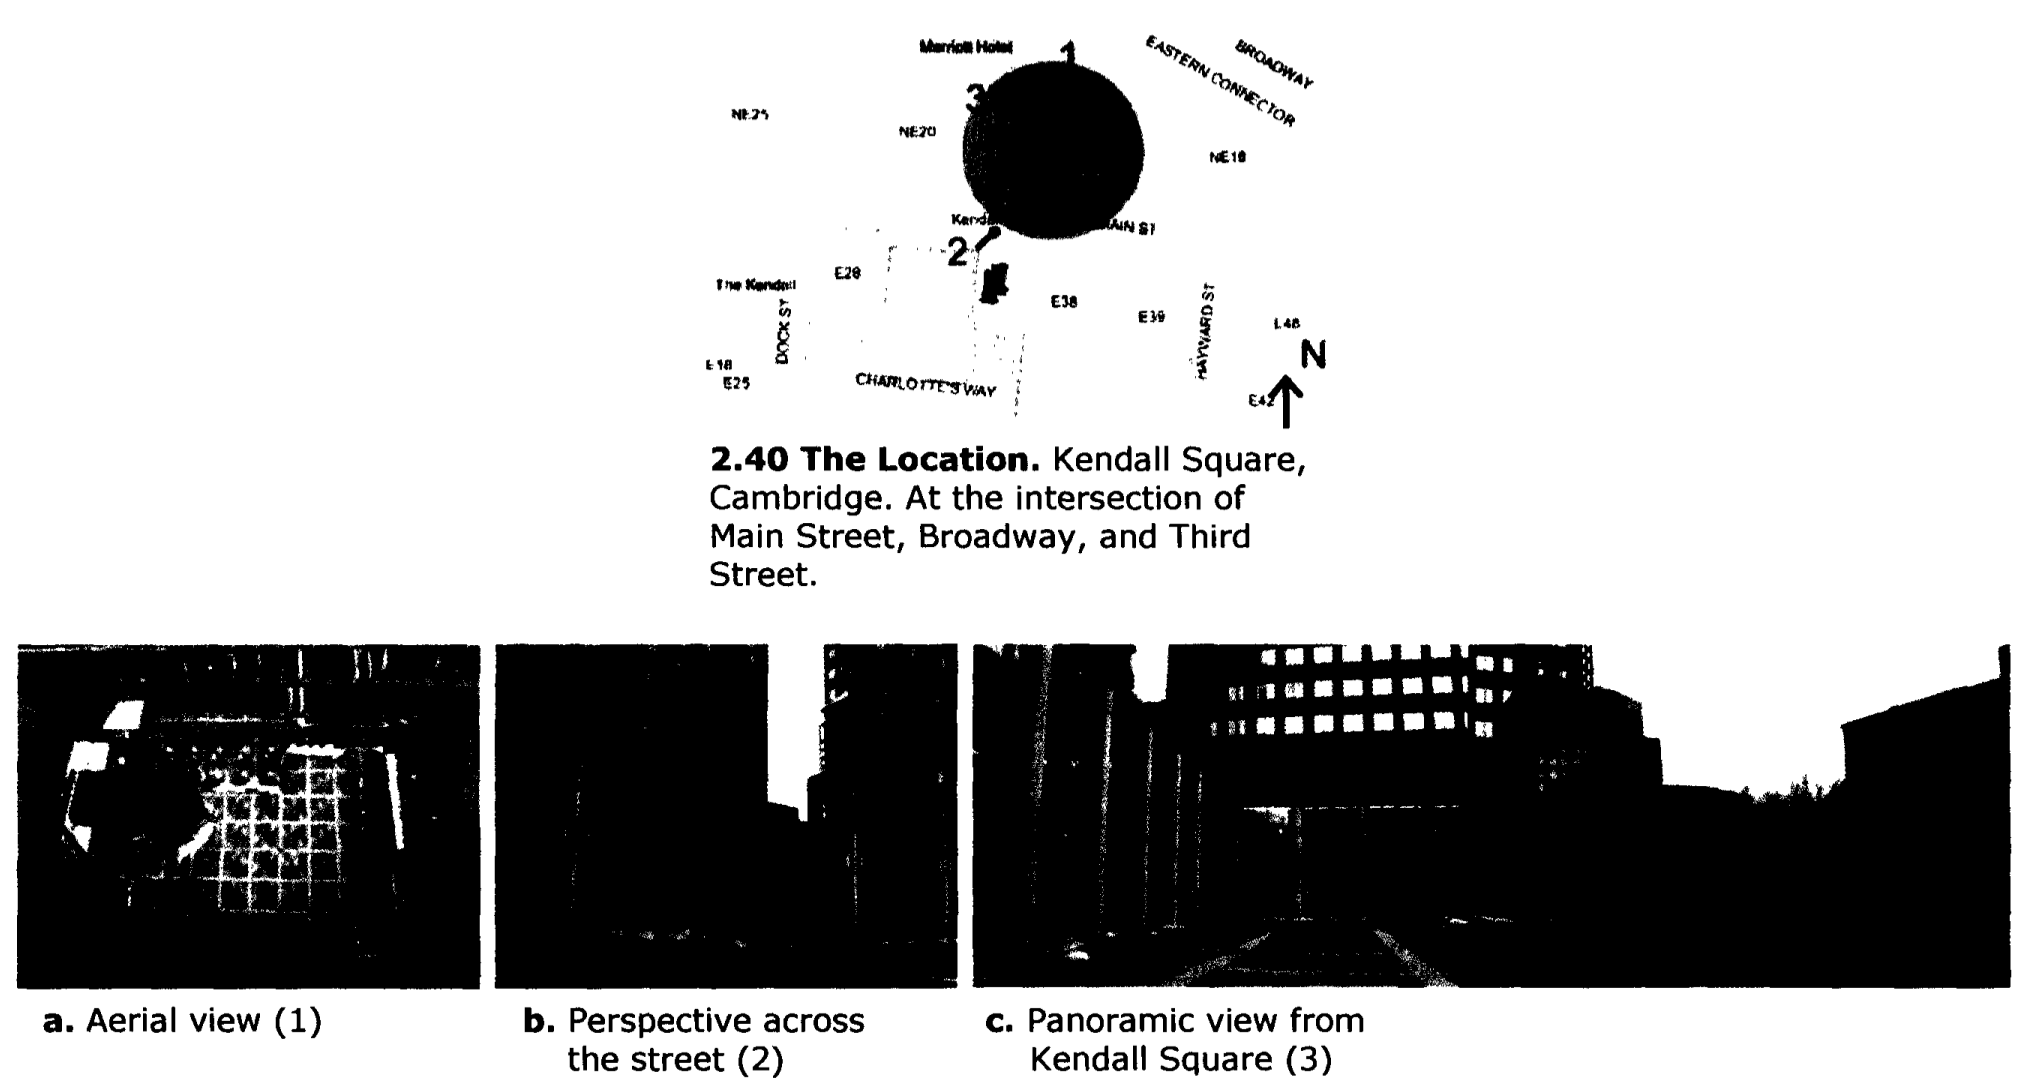
\includegraphics[width=\textwidth]{./Images/8-LocUrban}
\caption[Kendall Pavilion Location and Urban Context]{Location and Urban Context \cite{zulas04}}
\label{fig:KedLoc}
\end{figure}

\paragraph{The Design Intentions} 
\vspace{-0.3cm}
\begin{enumerate}
\item Generate an architectural skin.
\item Embed ``sensorial intelligence'' into the building, providing it with object recognition capabilities (surrounding buildings and pedestrian paths) and sun location responsiveness.
\item Embed ``structural intelligence'' into the building skin system, recognising and fixing potential structural instabilities, due to the fact that the building will suffer geometrical reconfigurations while responding to stimulus.
\end{enumerate}
\vspace{-0.4cm}
(See fig. \ref{fig:KenPavDesInt})

\begin{figure}[htbp]
\centering
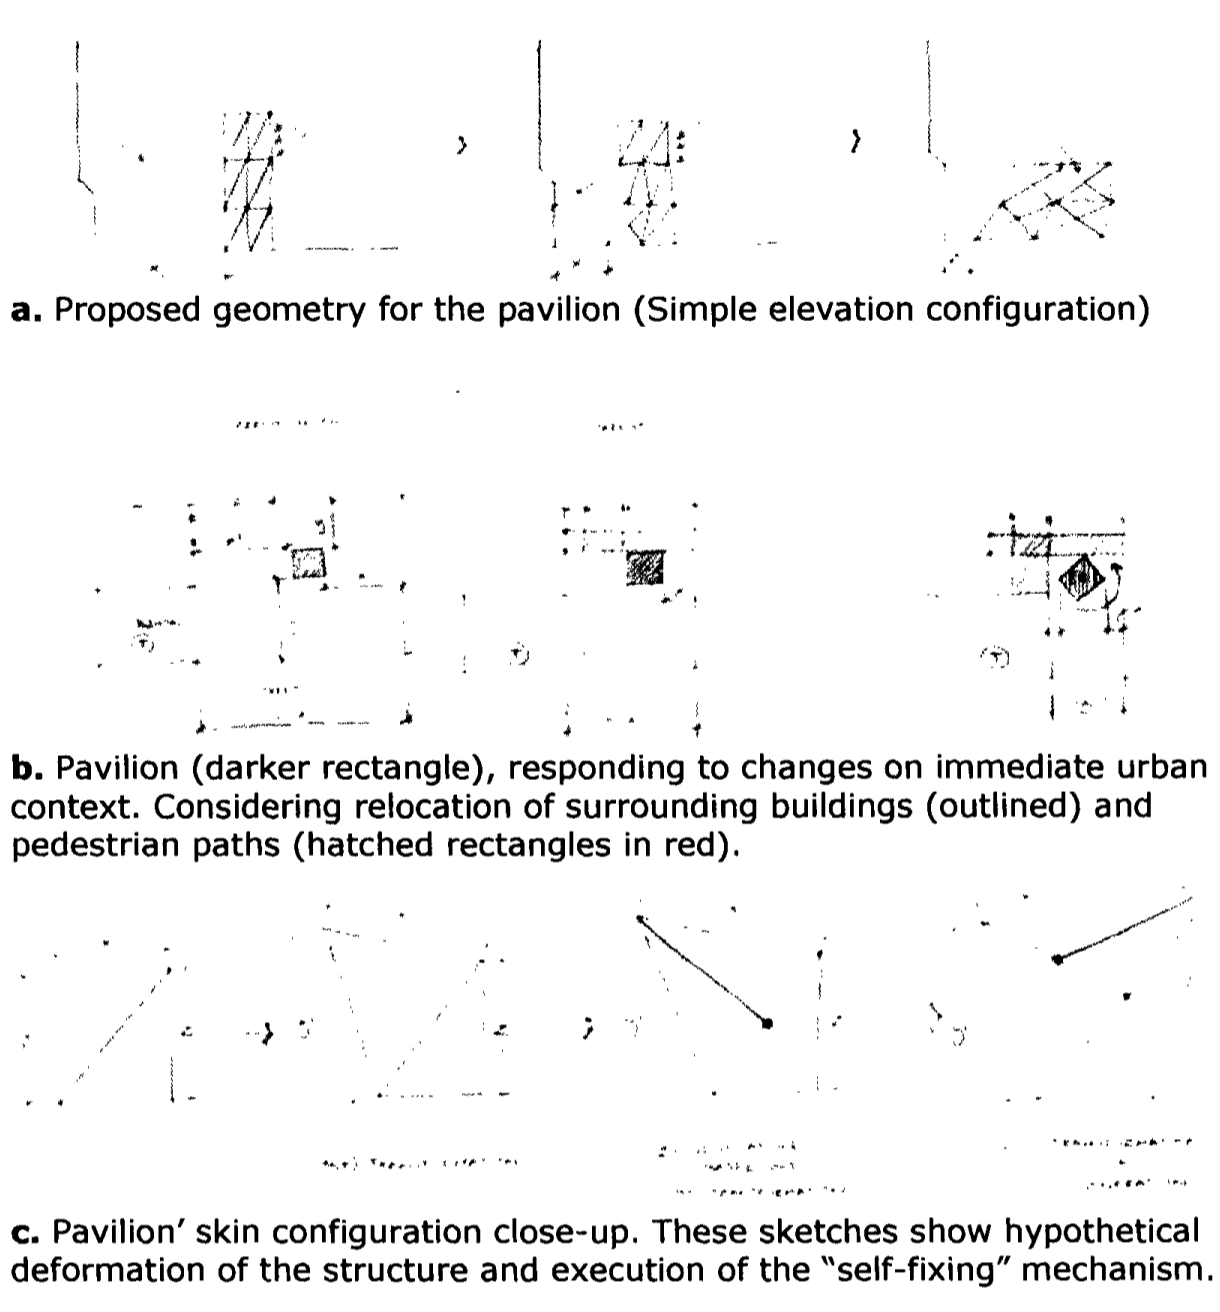
\includegraphics[width=0.7\textwidth]{./Images/9-DesInt}
\caption[Kendall Pavilion Design Intentions]{Kendall Pavilion Design Intentions \cite{zulas04}}
\label{fig:KenPavDesInt}
\end{figure}

\paragraph{The Mapping Process}

As the building will be corresponding to different stimulus, the cause and effect sequence had to be programmed, and four elements were selected as inputs:
\vspace{-0.3cm}
\begin{itemize}[nolistsep]
\item Program
\item Context
\item Environment
\item Designer Input
\end{itemize}
\vspace{-0.4cm}
(See fig. \ref{fig:MapProcs})

\begin{figure}[htbp]
\centering
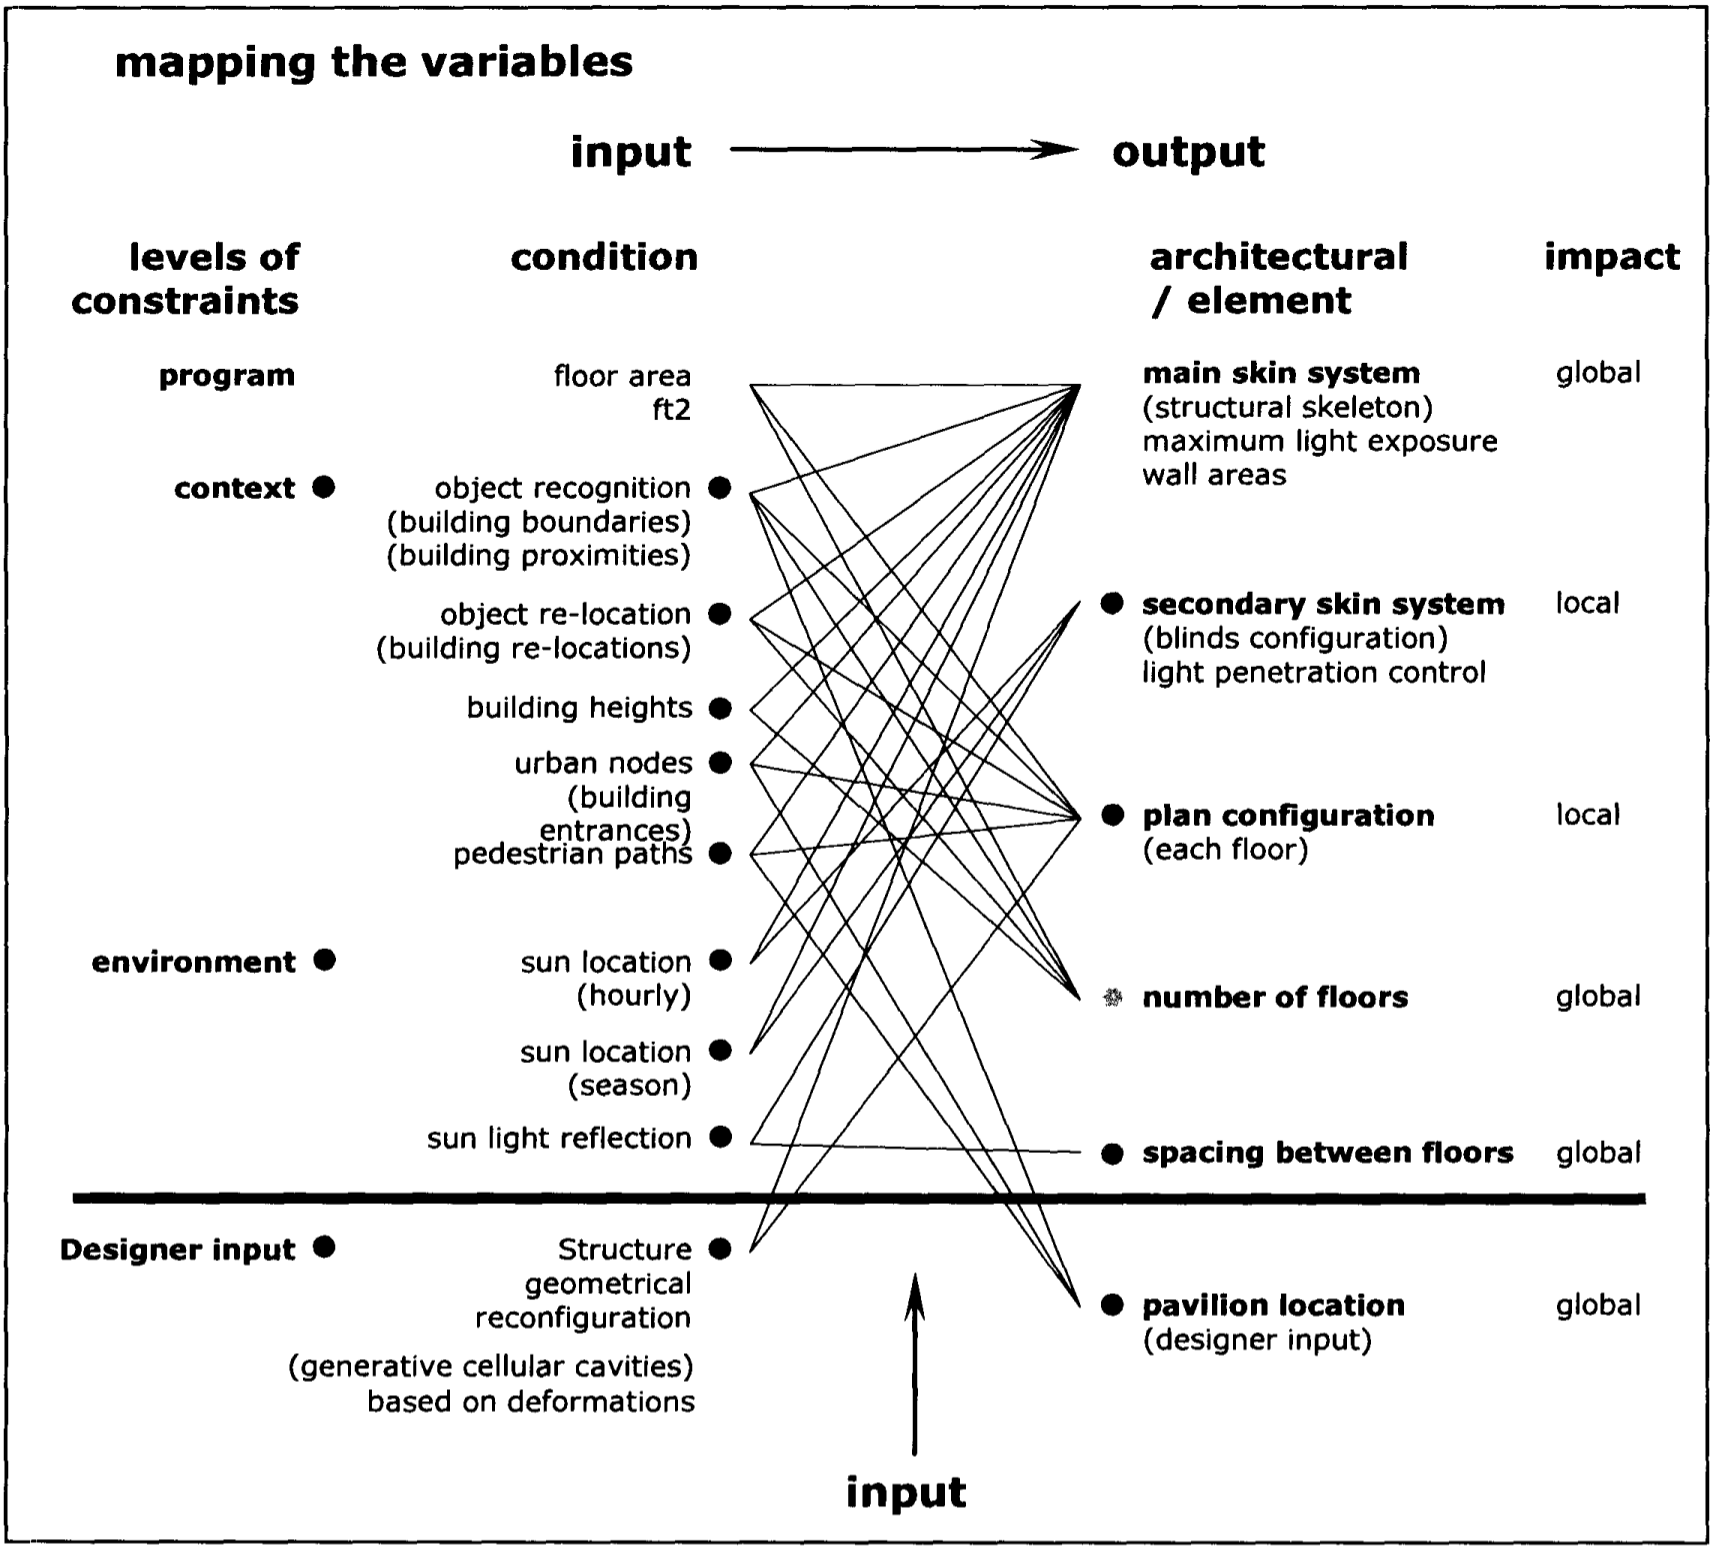
\includegraphics[width=\textwidth]{./Images/10-MapProcs}
\caption[Input/Output Mapping Process]{Input/Output Mapping Process \cite{zulas04}}
\label{fig:MapProcs}
\end{figure}

The author then continued to map the interrelationships of the architectural elements. This was due to the fact that each of the architectural elements would continue to affect each other in a continous loop indirectly (fig. \ref{fig:ArchElmLoop}).

\begin{figure}[htbp]
\centering
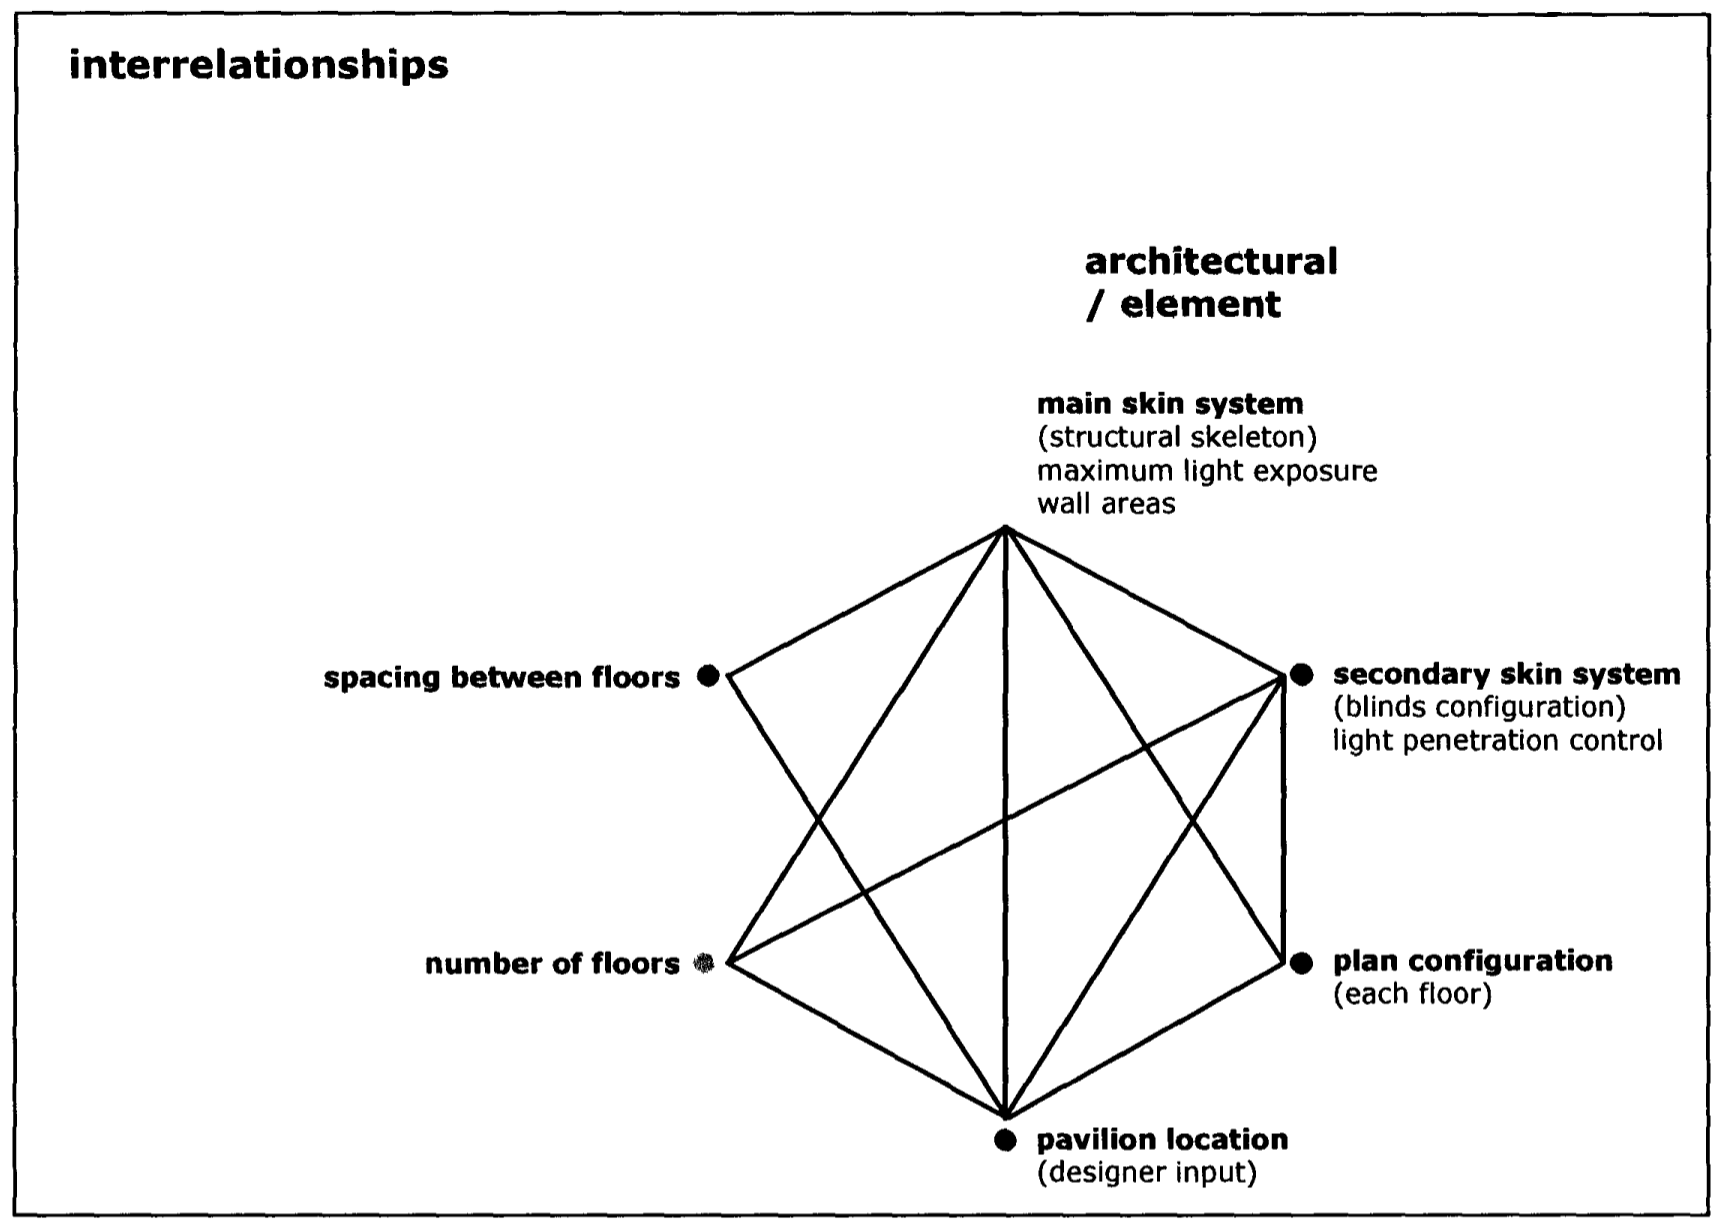
\includegraphics[width=\textwidth]{./Images/11-ArchElmLoop}
\caption[Architectural Elements Interrelationships]{Architecural Elements Interrelationships \cite{zulas04}}
\label{fig:ArchElmLoop}
\end{figure}

\paragraph{Control Mechanisms.}

Having defined the variables and mapping their interrelationships; the next step was to model the data and program the control algorithms. This process was inline with all the design intents mentioned earlier, namely: 
\begin{inparaenum}
\item ``embedding ``sensorial intellegence'' in order to achieve object recognition. To be achieved through contextual based conditional,
\item embedding ``smart flexibility'' allowing the user to intervene directly and freely with virtual objects throughout the design process. Implementing the concept of stretchable surfaces (to be further explained),
\item embedding ``structural intelligence in order to achieve specific self-fixing capabilities. Introducing the concept of emergence, to be implemented locally through a rule based approach (to be further explained).''
\end{inparaenum} \cite{zulas04}

The computational approaches that were used to tackle the three concepts stated above were: 

\begin{enumerate}[nolistsep]
\item Parametric representation of context
\item Parametric delimited action: Semi-automated human intervention
\item Generative emergence rules
\end{enumerate}

\subparagraph{Parametric representation of the context.} In order for the system to be ``adaptive'' and ``responsive'', the context should be variable, and therefore parameterized. In the earlier work by the autor (refer to section \ref{sec:AdptPav}) the stimulus to which the building had responded was the sun and its movement. Here however, the whole context of buildins, roads and the rest of the stiumuli mentioned earlier will affect the buildings response (see fig. \ref{fig:ParametricKendallSq}).

\begin{figure}[htbp]
\centering
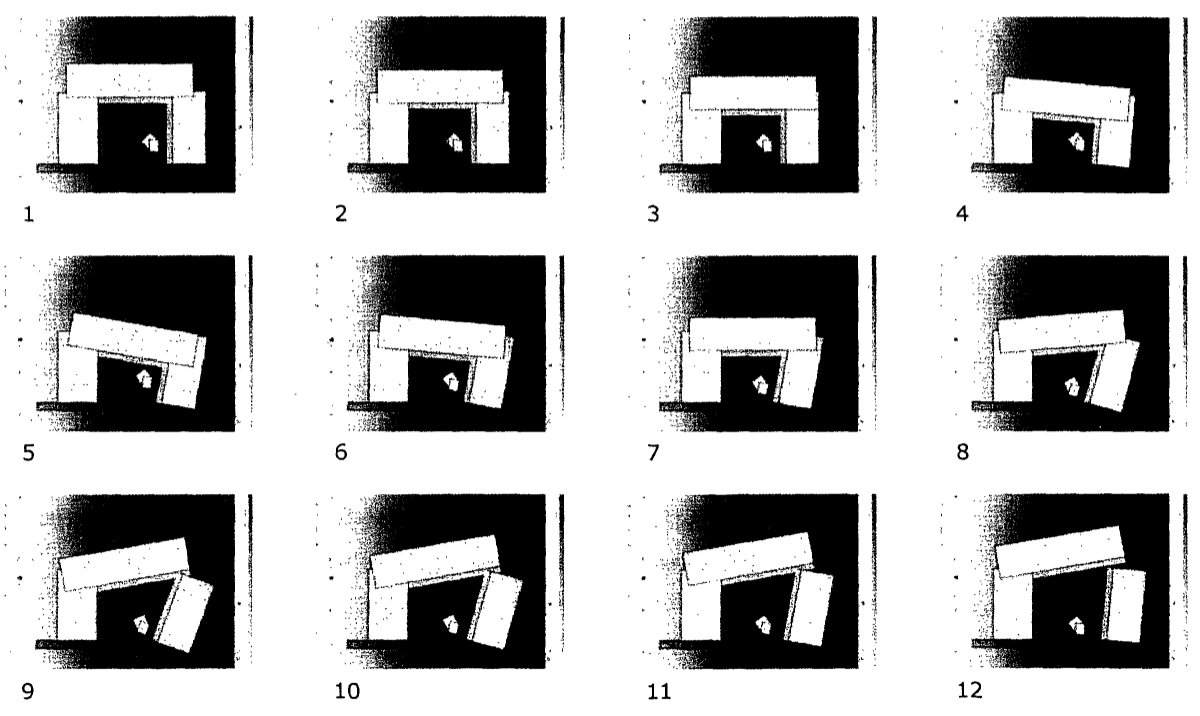
\includegraphics[width=\textwidth]{./Images/12-ParametricContext}
\caption[Parametric Context]{A plan view of the Kendall Square area being manipulated to generate different context through parametric controls \cite {zulas04}}
\label{fig:ParametricKendallSq}
\end{figure}

\begin{figure}[htbp]
\centering
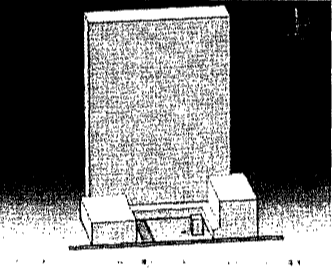
\includegraphics[width=0.4\textwidth]{./Images/13-KendallIsometric}
\caption[Kendall Square Isometric]{An isometric of the Kendall Square \cite{zulas04}}
\label{fig:KendallIsom}
\end{figure}

The parametrization of the context was achieved by applying a stretchable two-dimensional grid, or net, of lines on the surrounding buildings and pedestrian paths. The method is referred to by the author as manipulation through ``stretchable surfaces''.

\subparagraph{Delimited Action: Semi-automated Human Intervention.}
The ``stretchable surfaces'' concept was further incorporated into the system by making adaption of the pavilion respond to any changes in the grid, which would act as a guide to the programmed adaption algorithm, while allowing direct adjustments to the grid by the designer; hence, a ``semi-automated'' human intervention.

\subparagraph{Generative Emergence Rules.} As mentioned earlier in this chapter; draughting and modelling programs usually provide generative modelling through scripting (end-user programming languages). In this case the author \cite{zuals04} utilized the scripting capabilities of CATIA (parametric modelling application). The emergence rule acts as a form of ``structural intelligence'' (a concept described earlier) where the rule identifies the length of two sides of the basic composition of the pavilion's main structure; which if they are exceeded the system will automatically add an emergent structural element to preserve structural integrity. The script used is shown in fig. \ref{fig:EmergRuleScr}.

\begin{figure}[htbp]
\centering
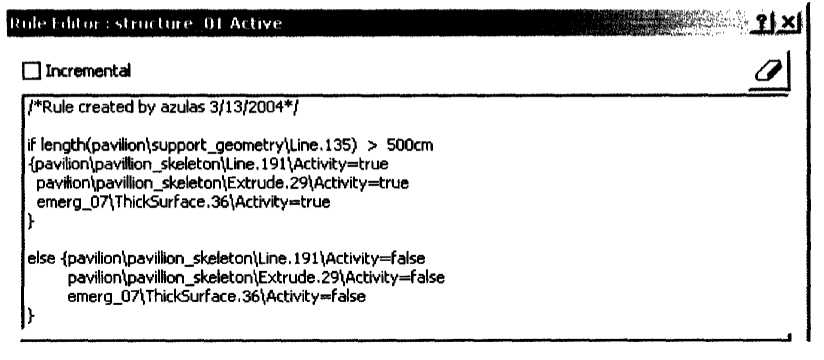
\includegraphics[width=0.7\textwidth]{./Images/14-EmergRuleScr}
\caption[Emergence Rule Script]{A screen capture of the script used in CATIA to apply the emergence rule \cite{zulas04}}
\label{fig:EmergRuleScr}
\end{figure}


